\chapter{Anhang}\label{ch:appendix}

\begin{figure}[htp]
    \centering
    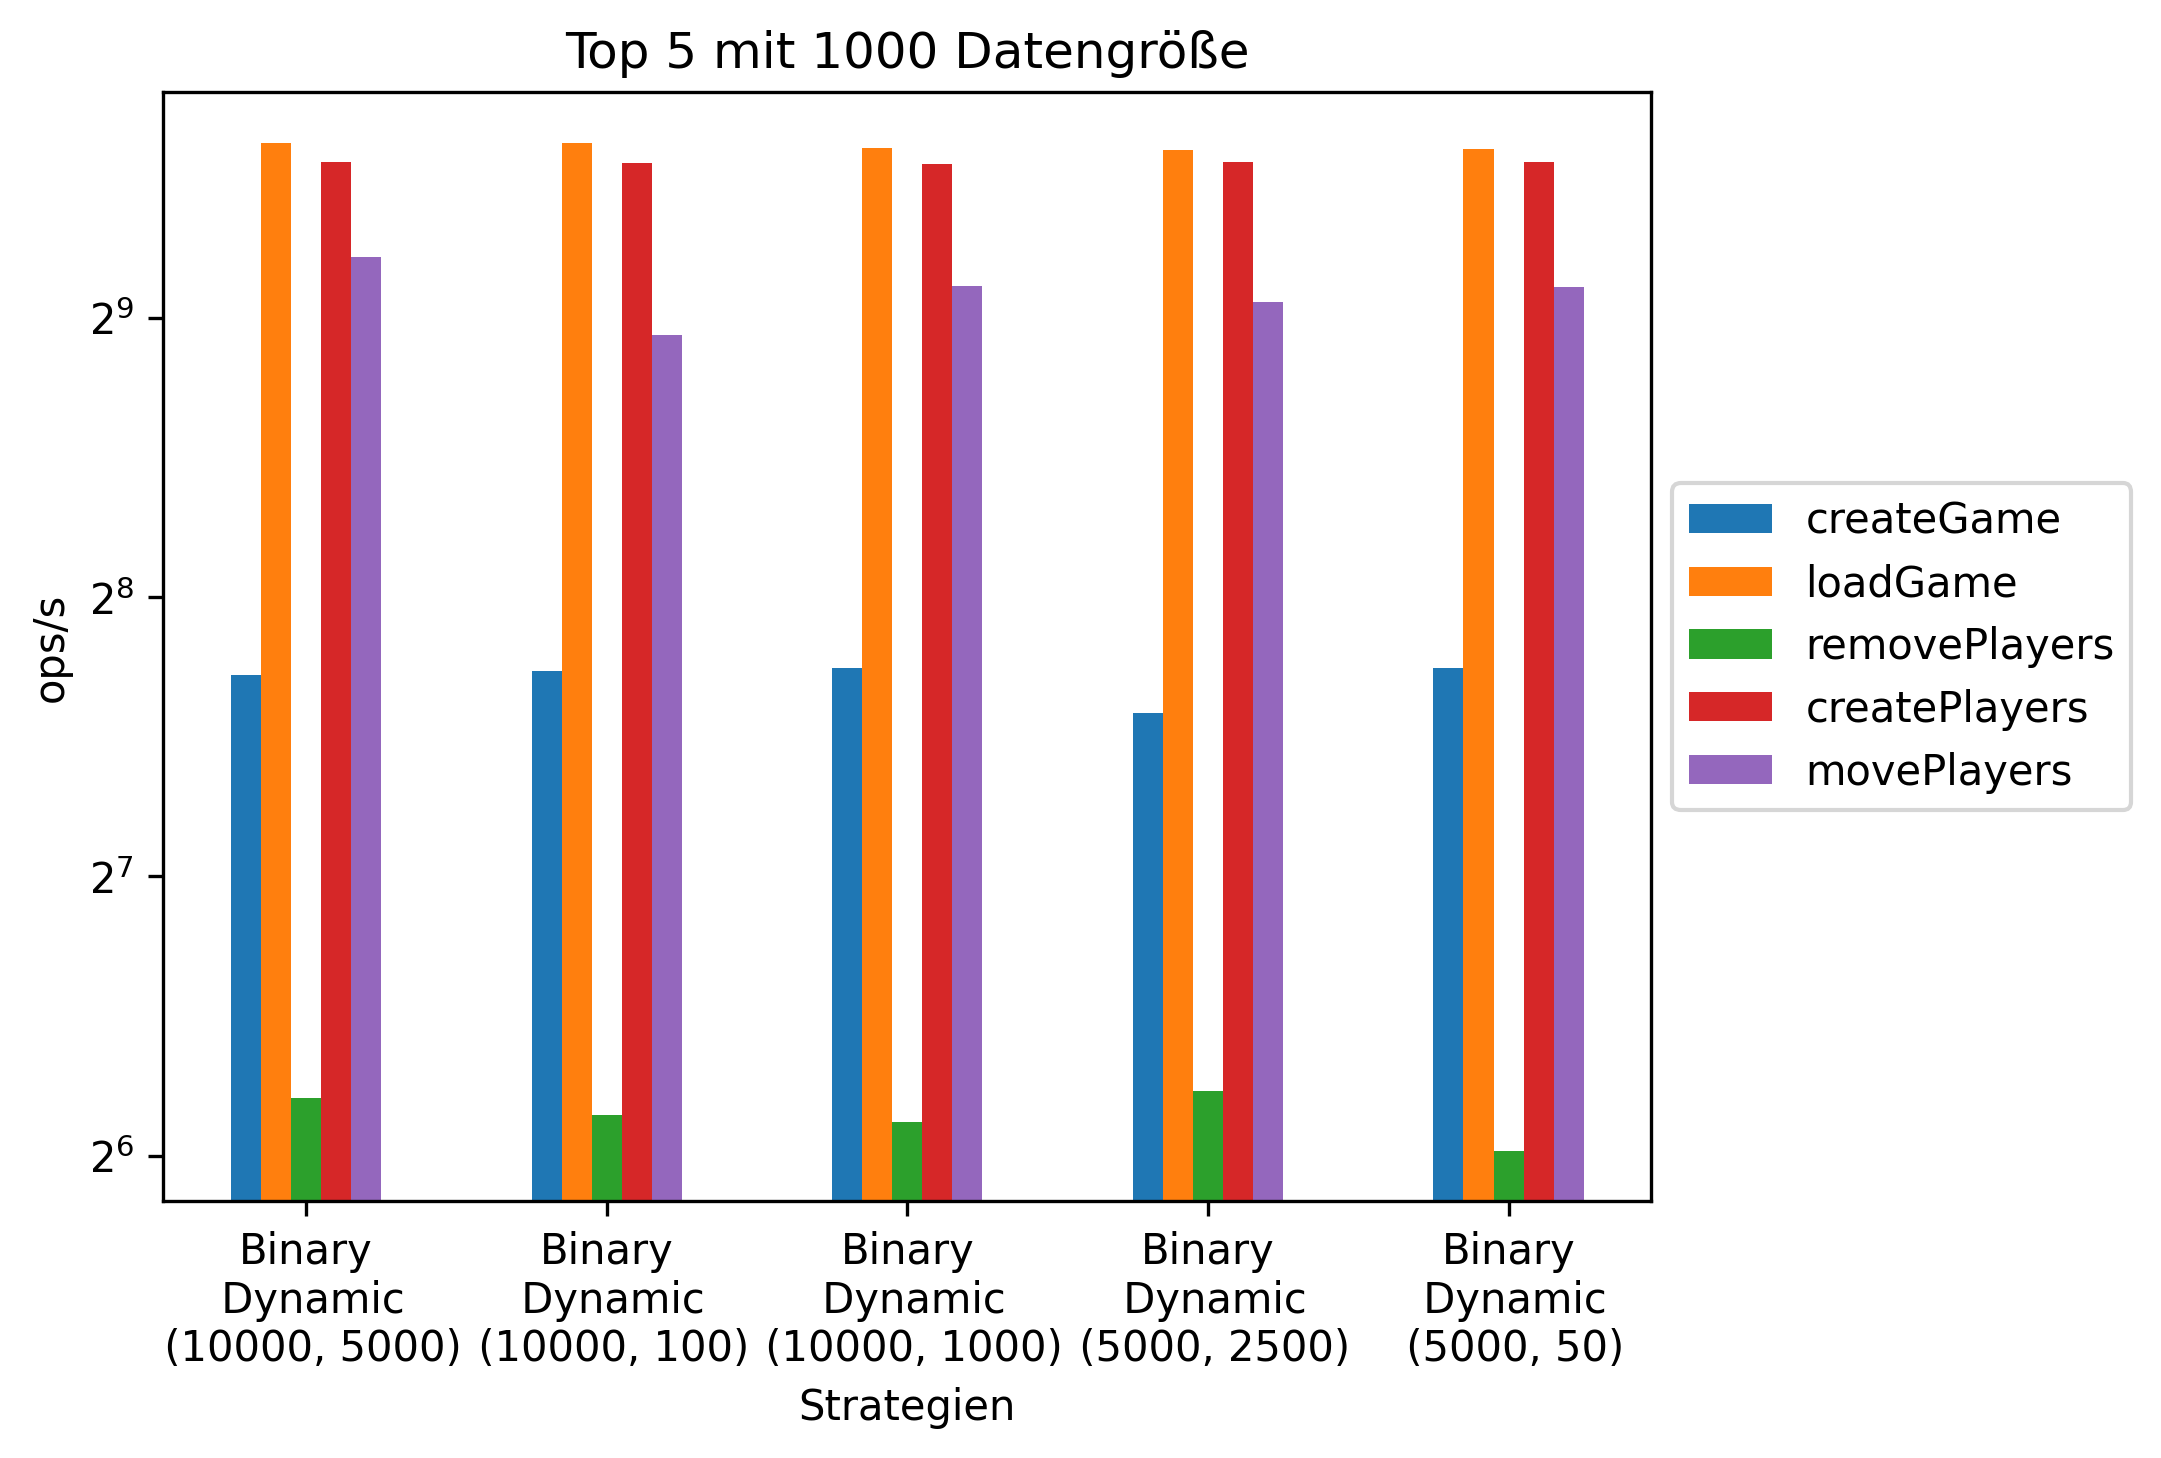
\includegraphics[width=0.7\textwidth]{images/plots/1000.png}
    \caption{Beste Strategien bei einer Daten-Anzahl von 1000}
    \label{fig:smallDataCount}
\end{figure}

\begin{figure}[htp]
    \centering
    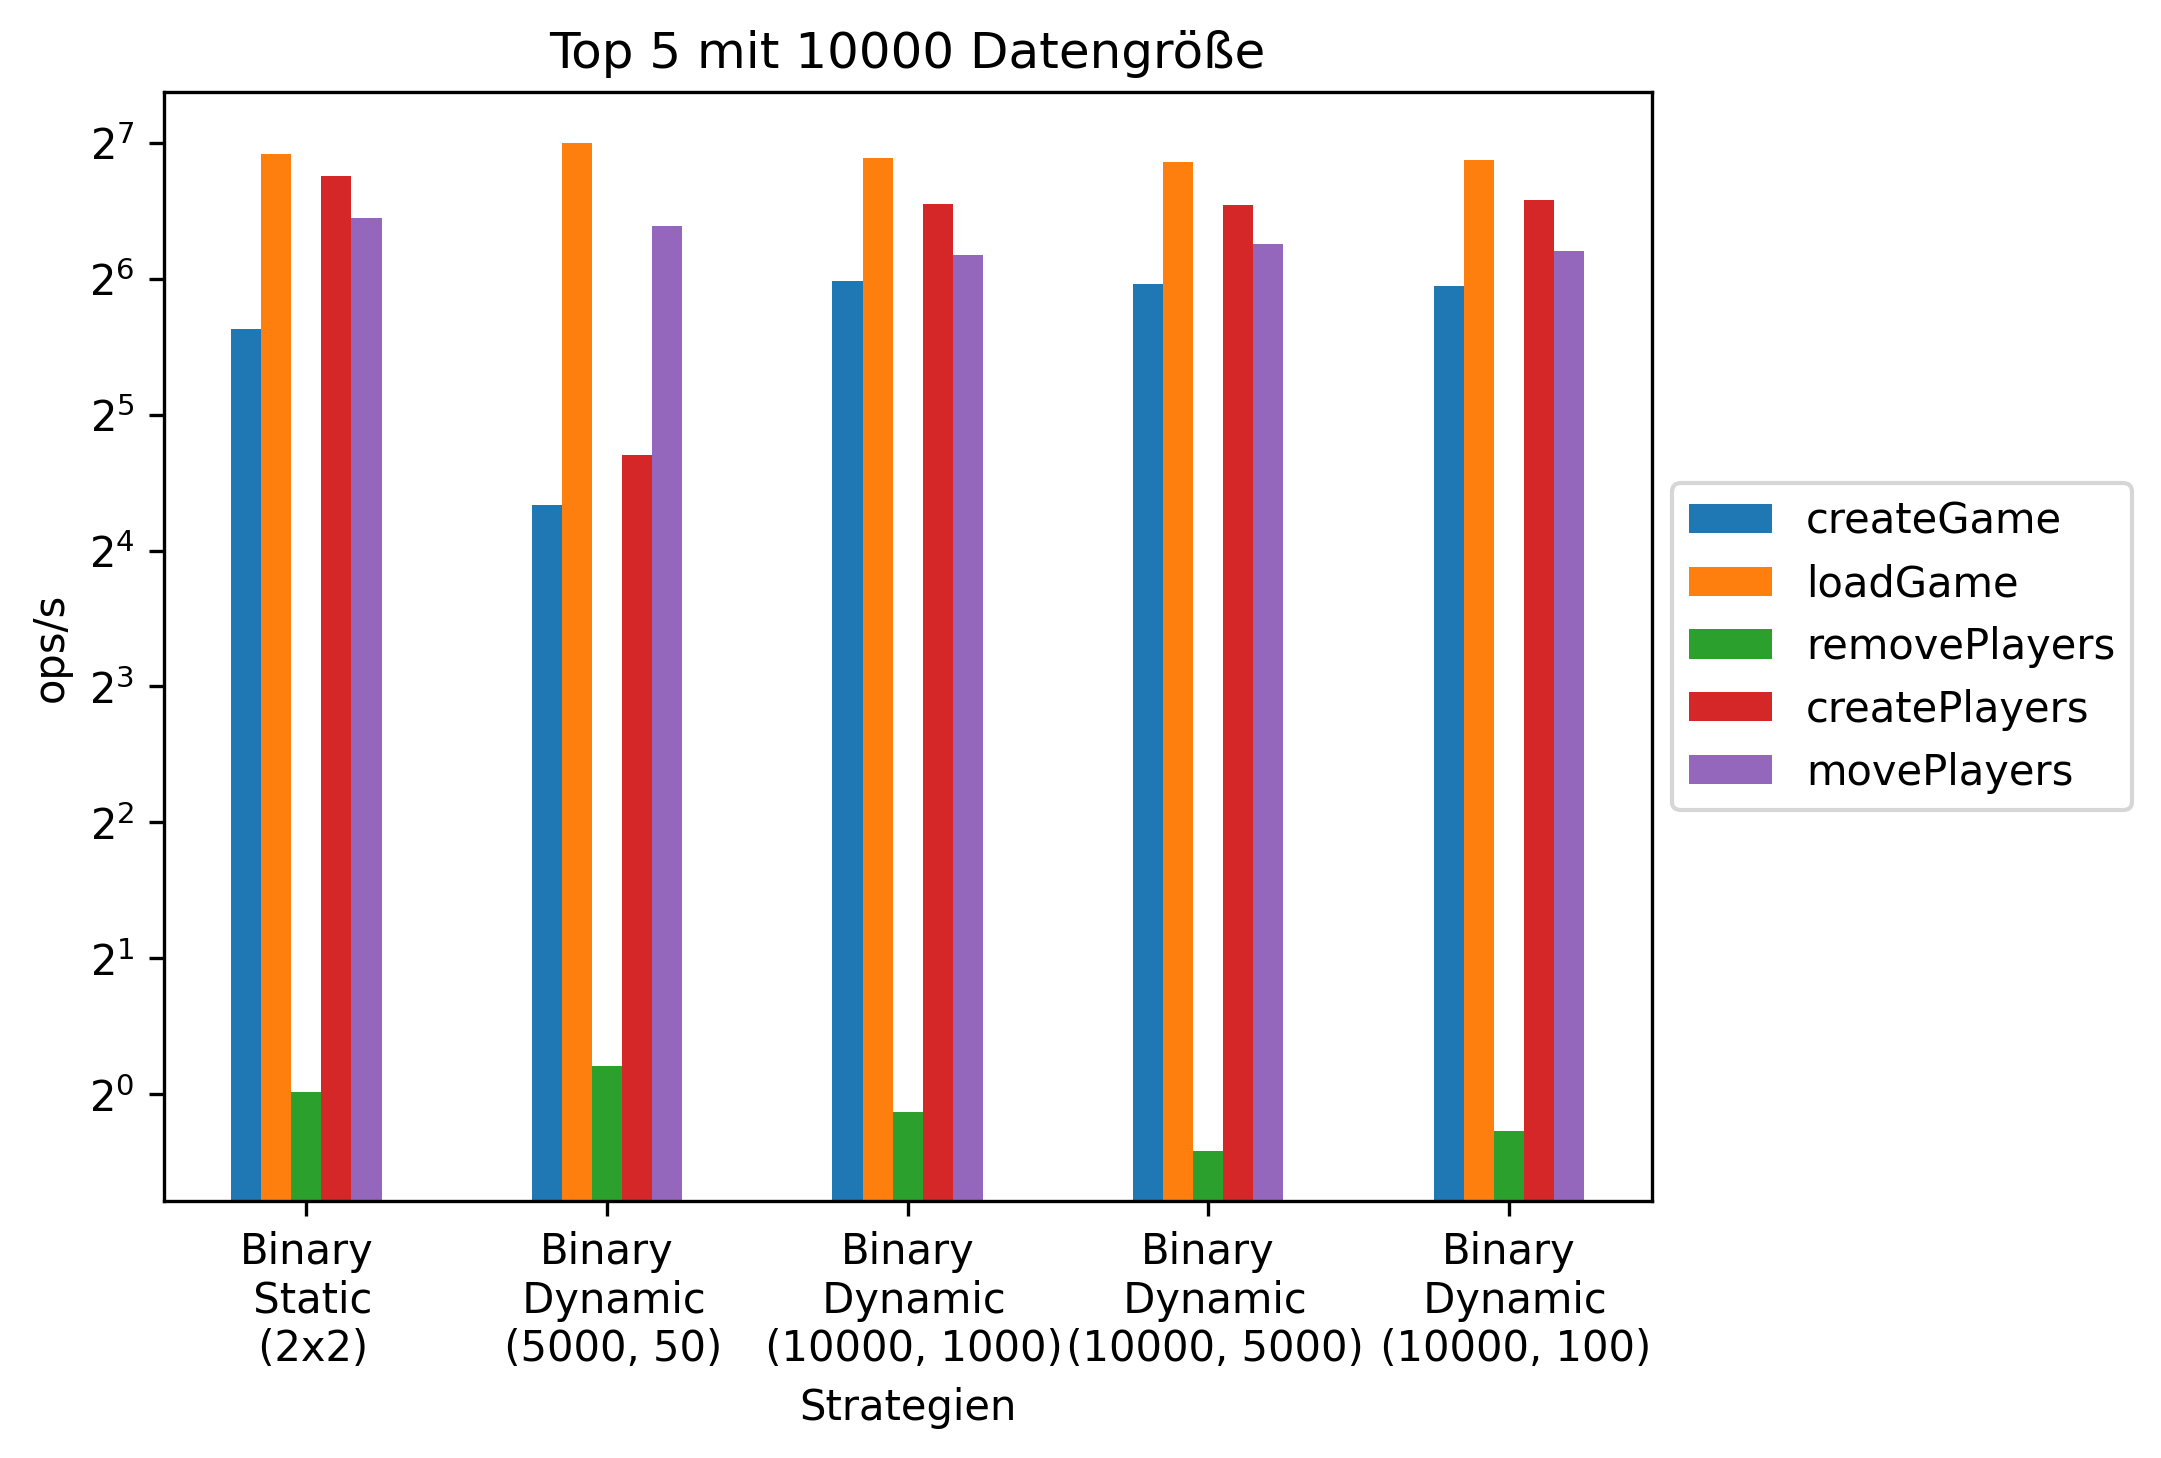
\includegraphics[width=0.7\textwidth]{images/plots/10000.png}
    \caption{Beste Strategien bei einer Daten-Anzahl von 10000}
    \label{fig:middleDataCount}
\end{figure}

\begin{figure}[htp]
    \centering
    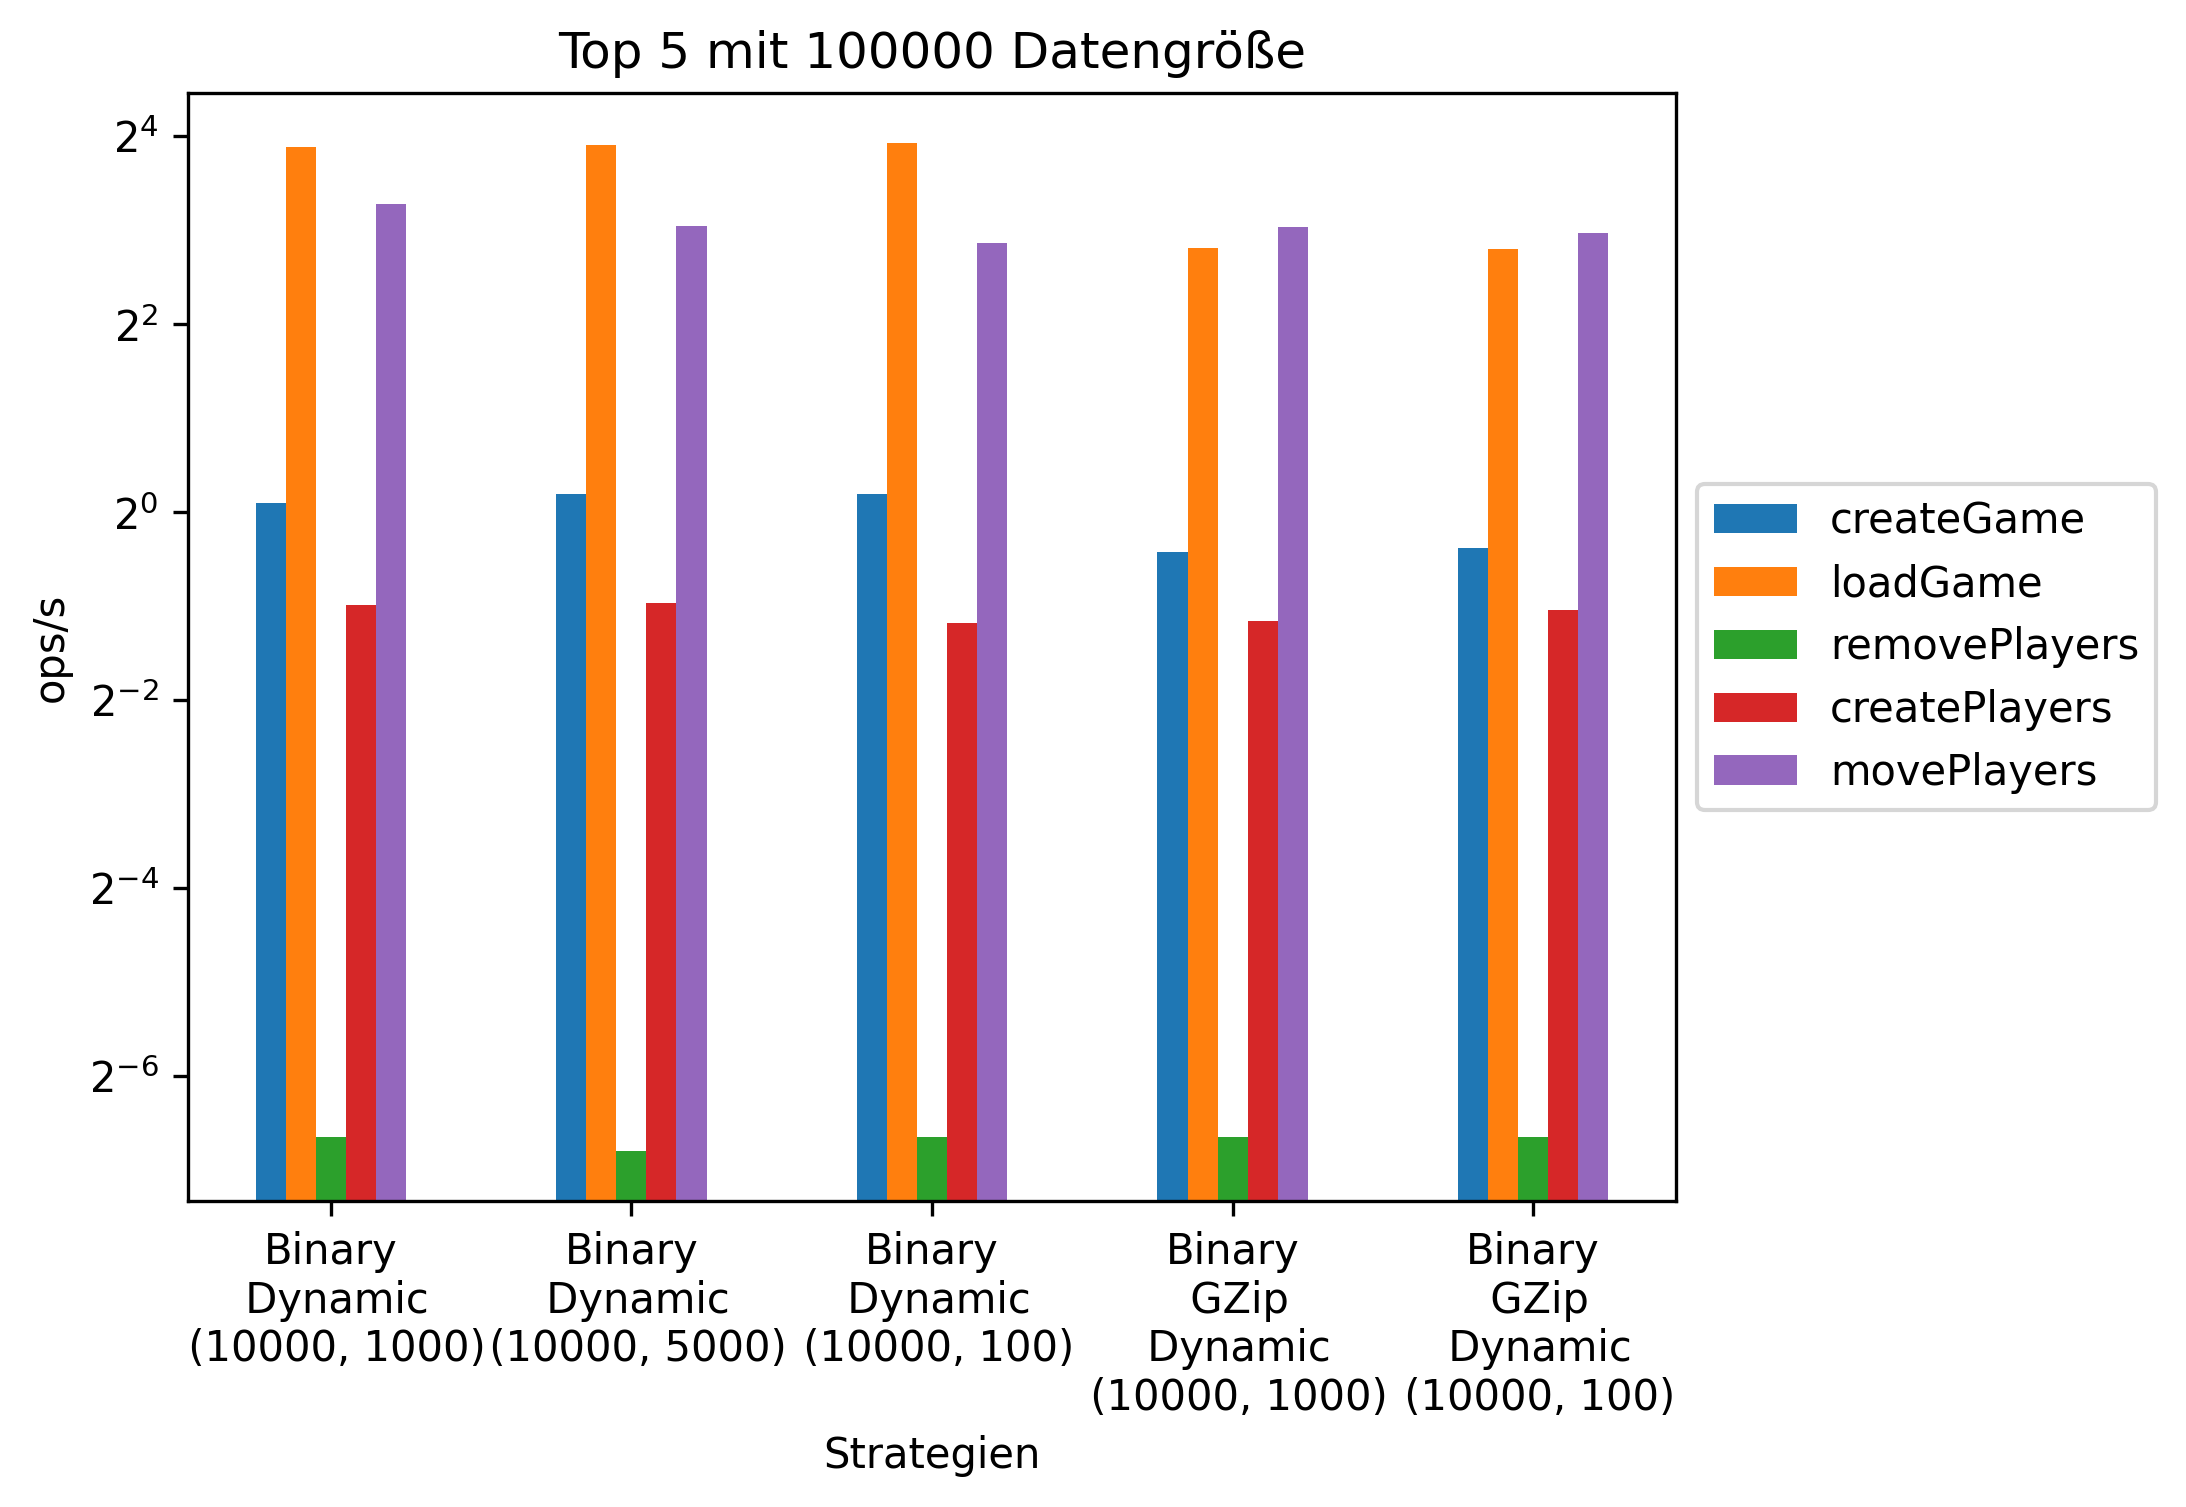
\includegraphics[width=0.7\textwidth]{images/plots/100000.png}
    \caption{Beste Strategien bei einer Daten-Anzahl von 100000}
    \label{fig:bigDataCount}
\end{figure}

\begin{figure}[htp]
    \centering
    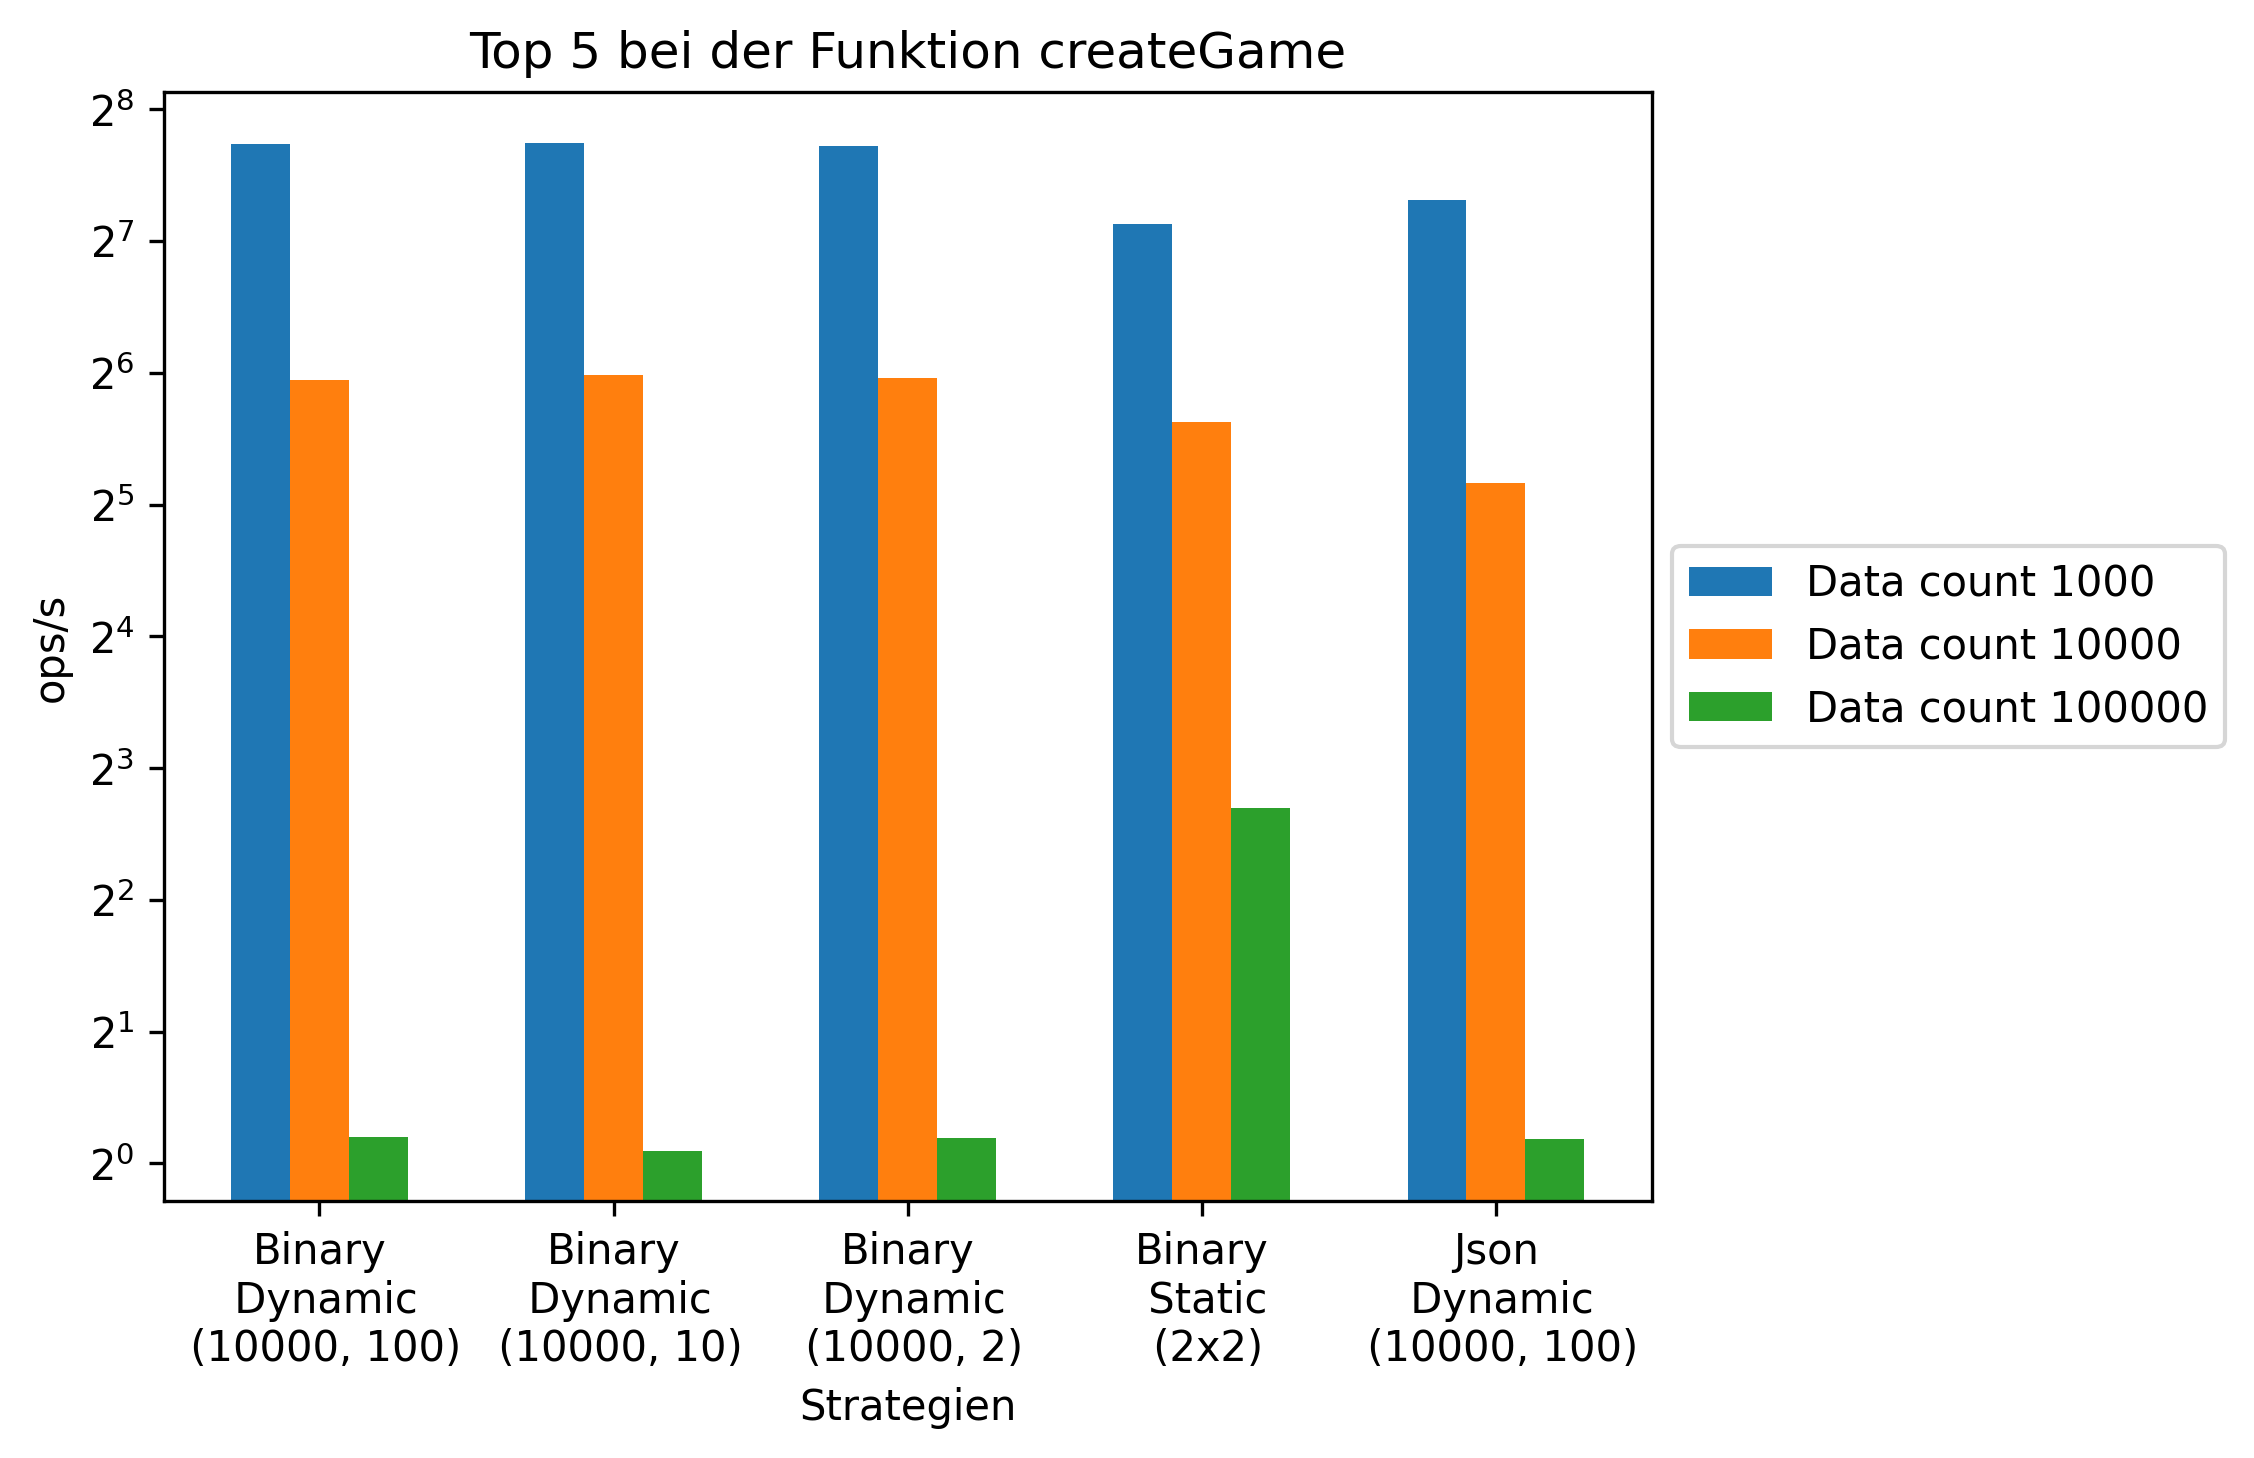
\includegraphics[width=0.7\textwidth]{images/plots/createGame.png}
    \caption{Beste Strategien für die Funktion createGame}
    \label{fig:createGame}
\end{figure}

\begin{figure}[htp]
    \centering
    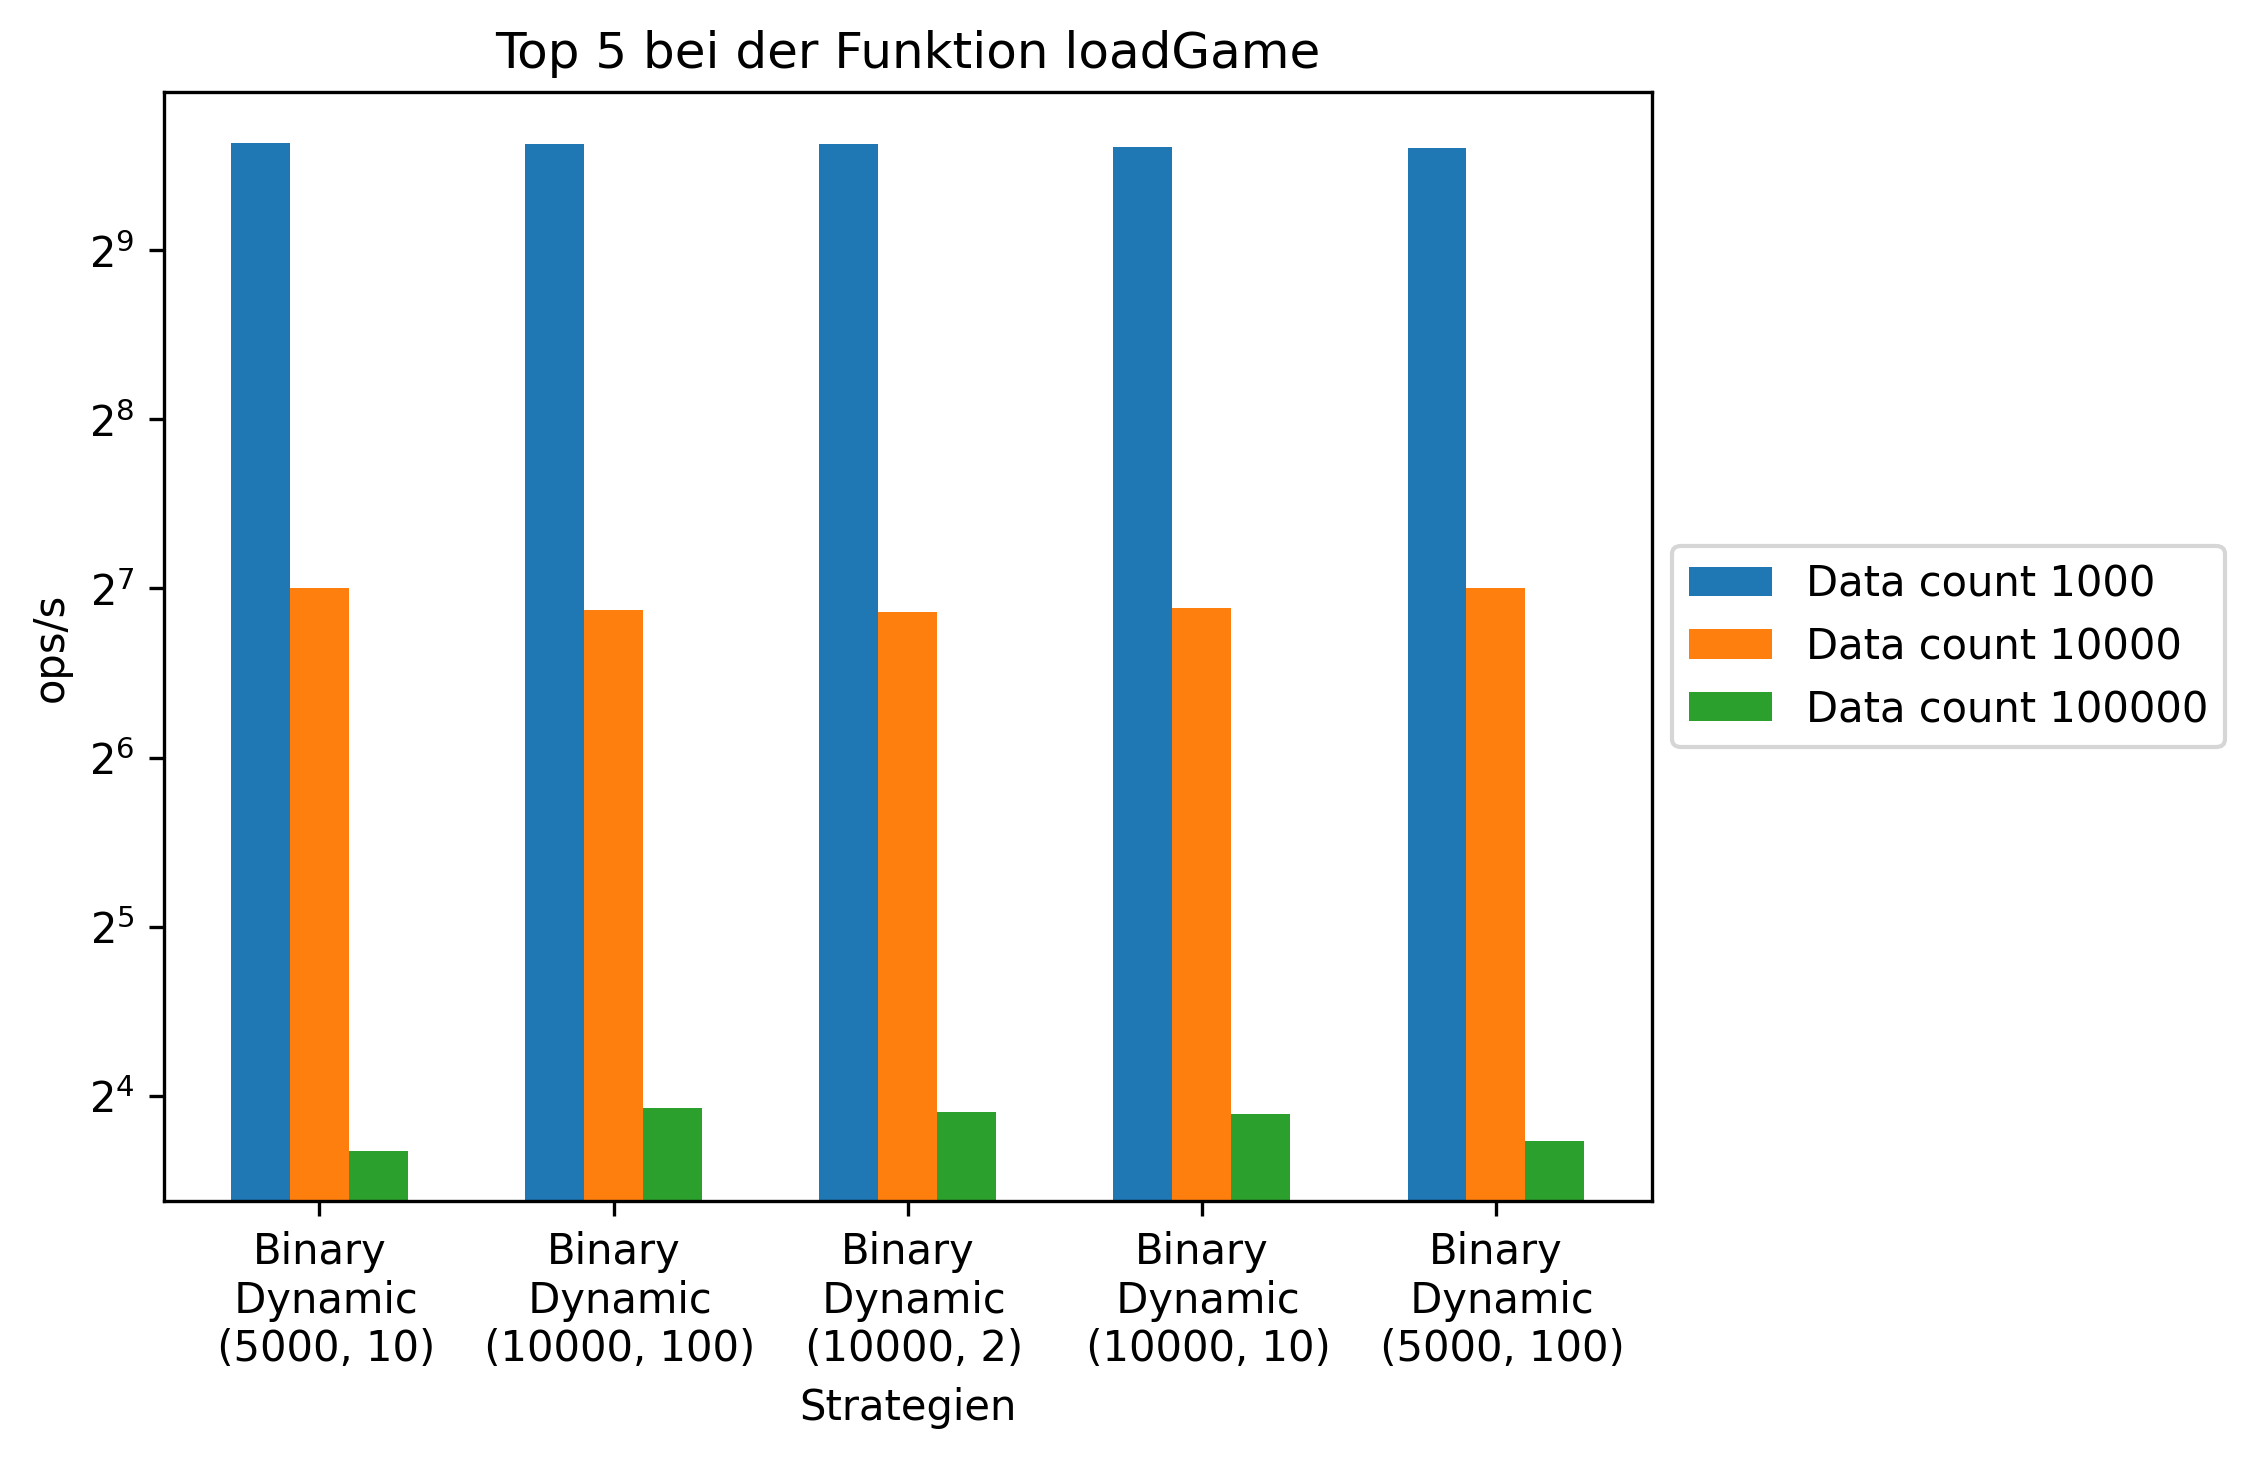
\includegraphics[width=0.7\textwidth]{images/plots/loadGame.png}
    \caption{Beste Strategien für die Funktion loadGame}
    \label{fig:loadGame}
\end{figure}

\begin{figure}[htp]
    \centering
    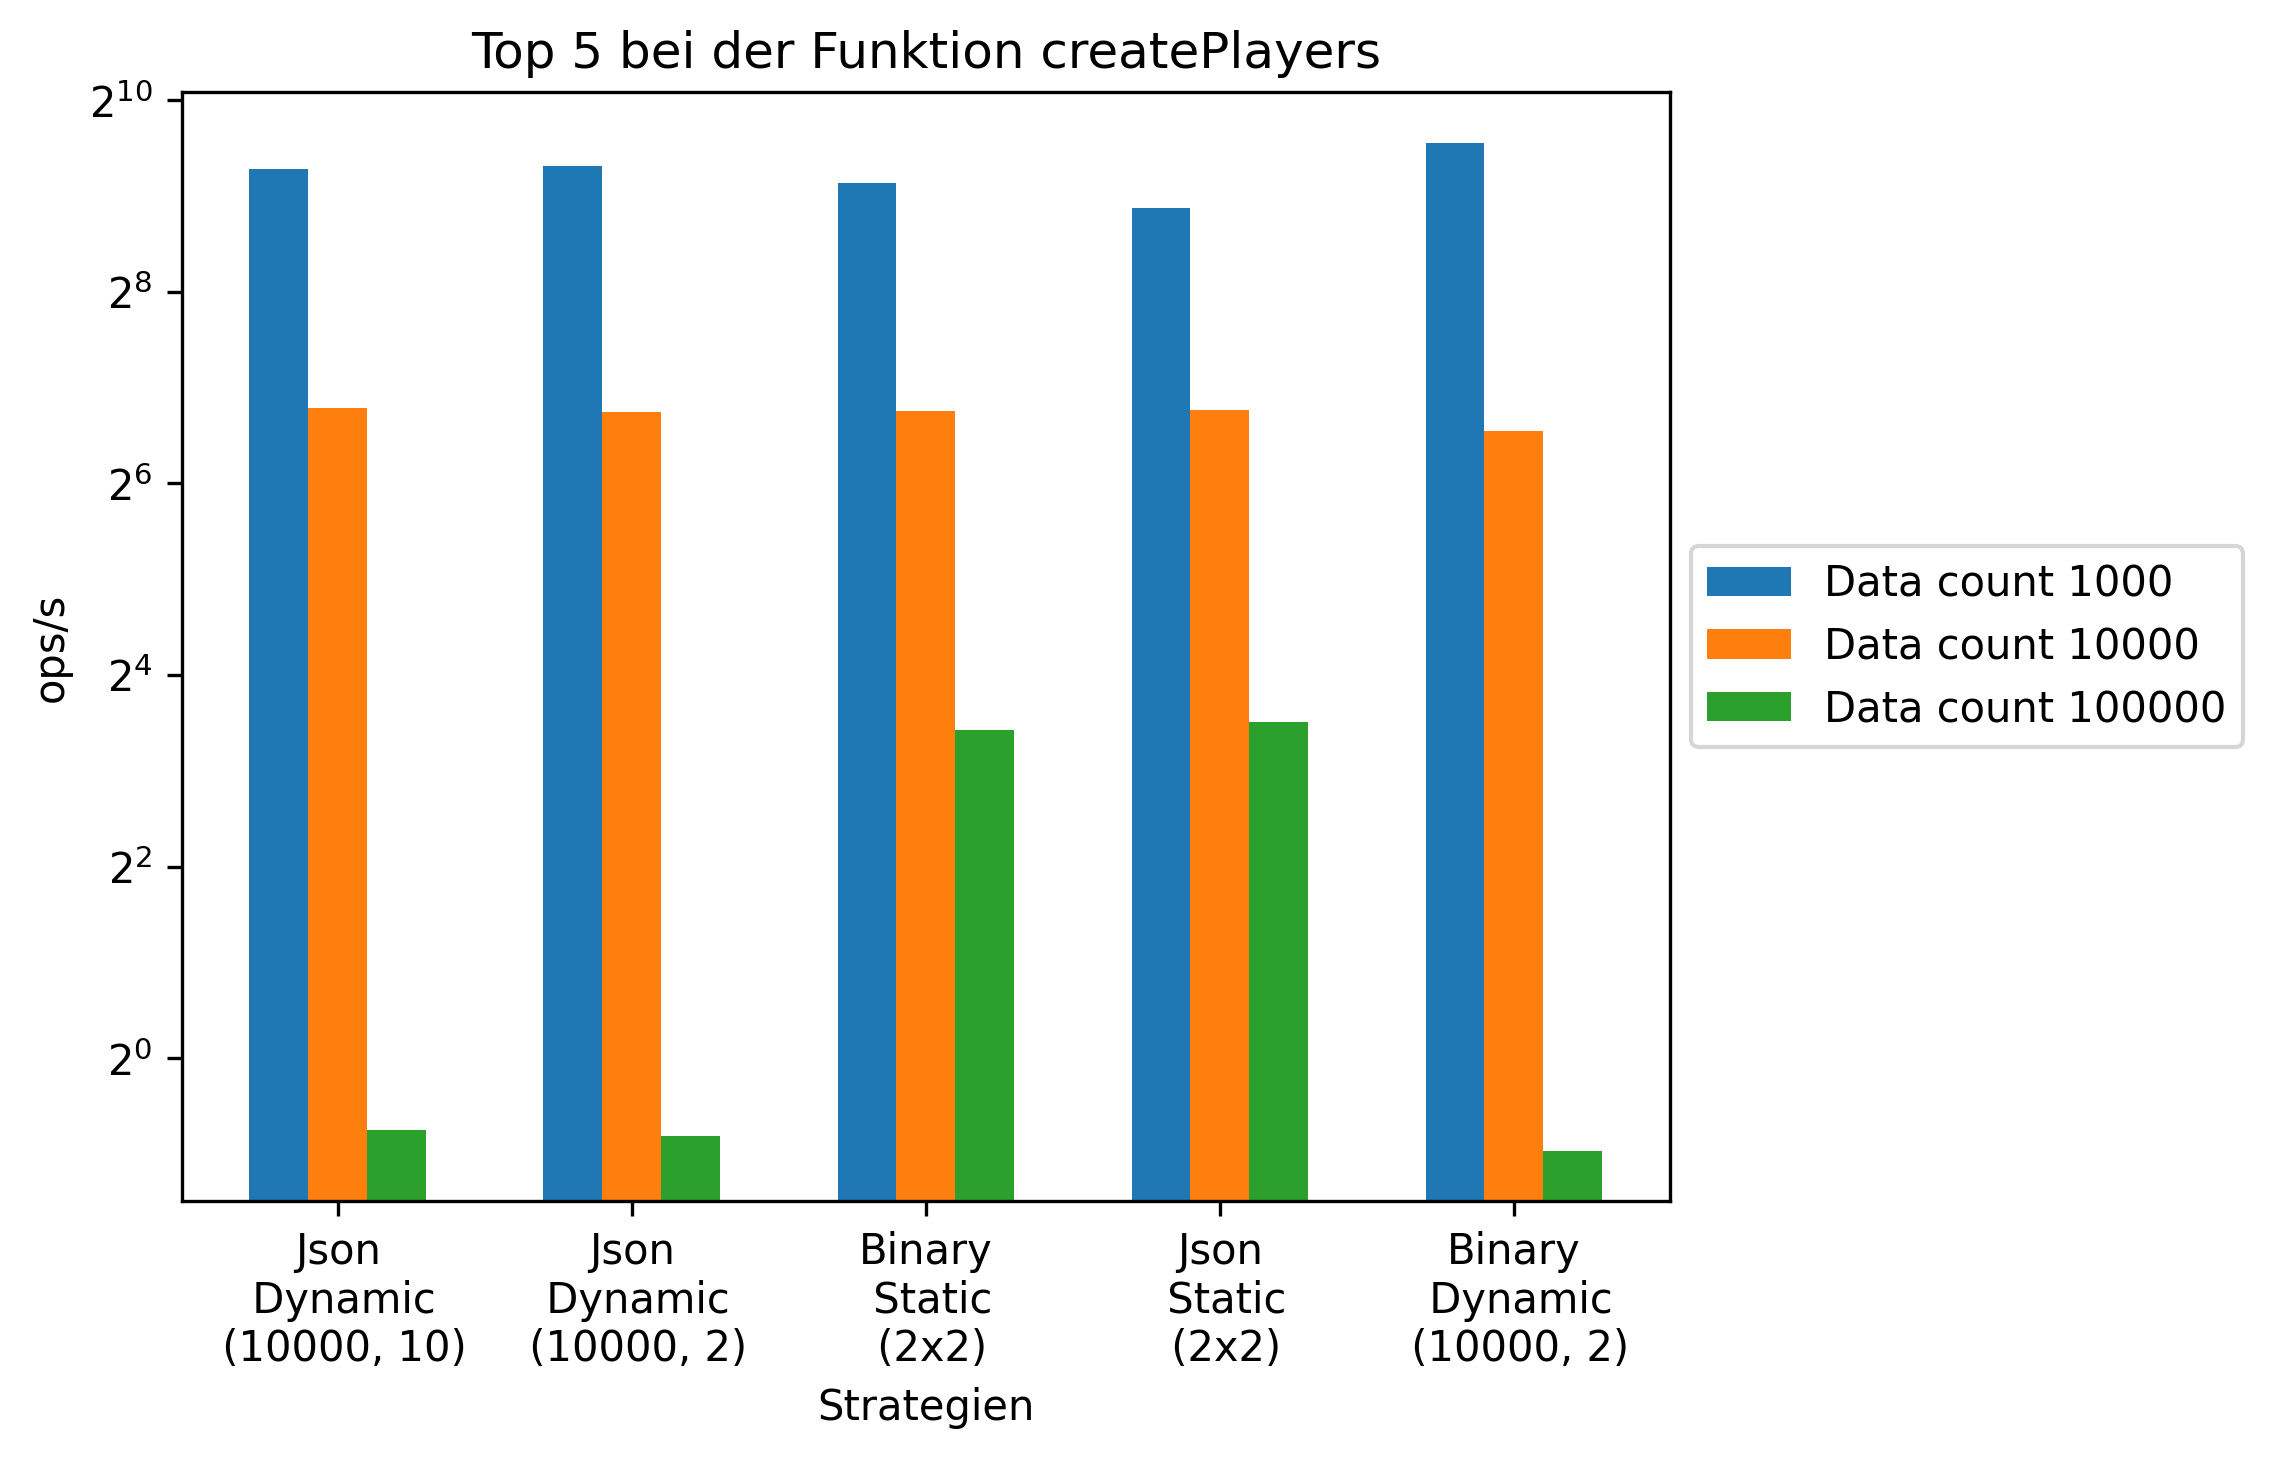
\includegraphics[width=0.7\textwidth]{images/plots/createPlayers.png}
    \caption{Beste Strategien für die Funktion createPlayers}
    \label{fig:createPlayers}
\end{figure}

\begin{figure}[htp]
    \centering
    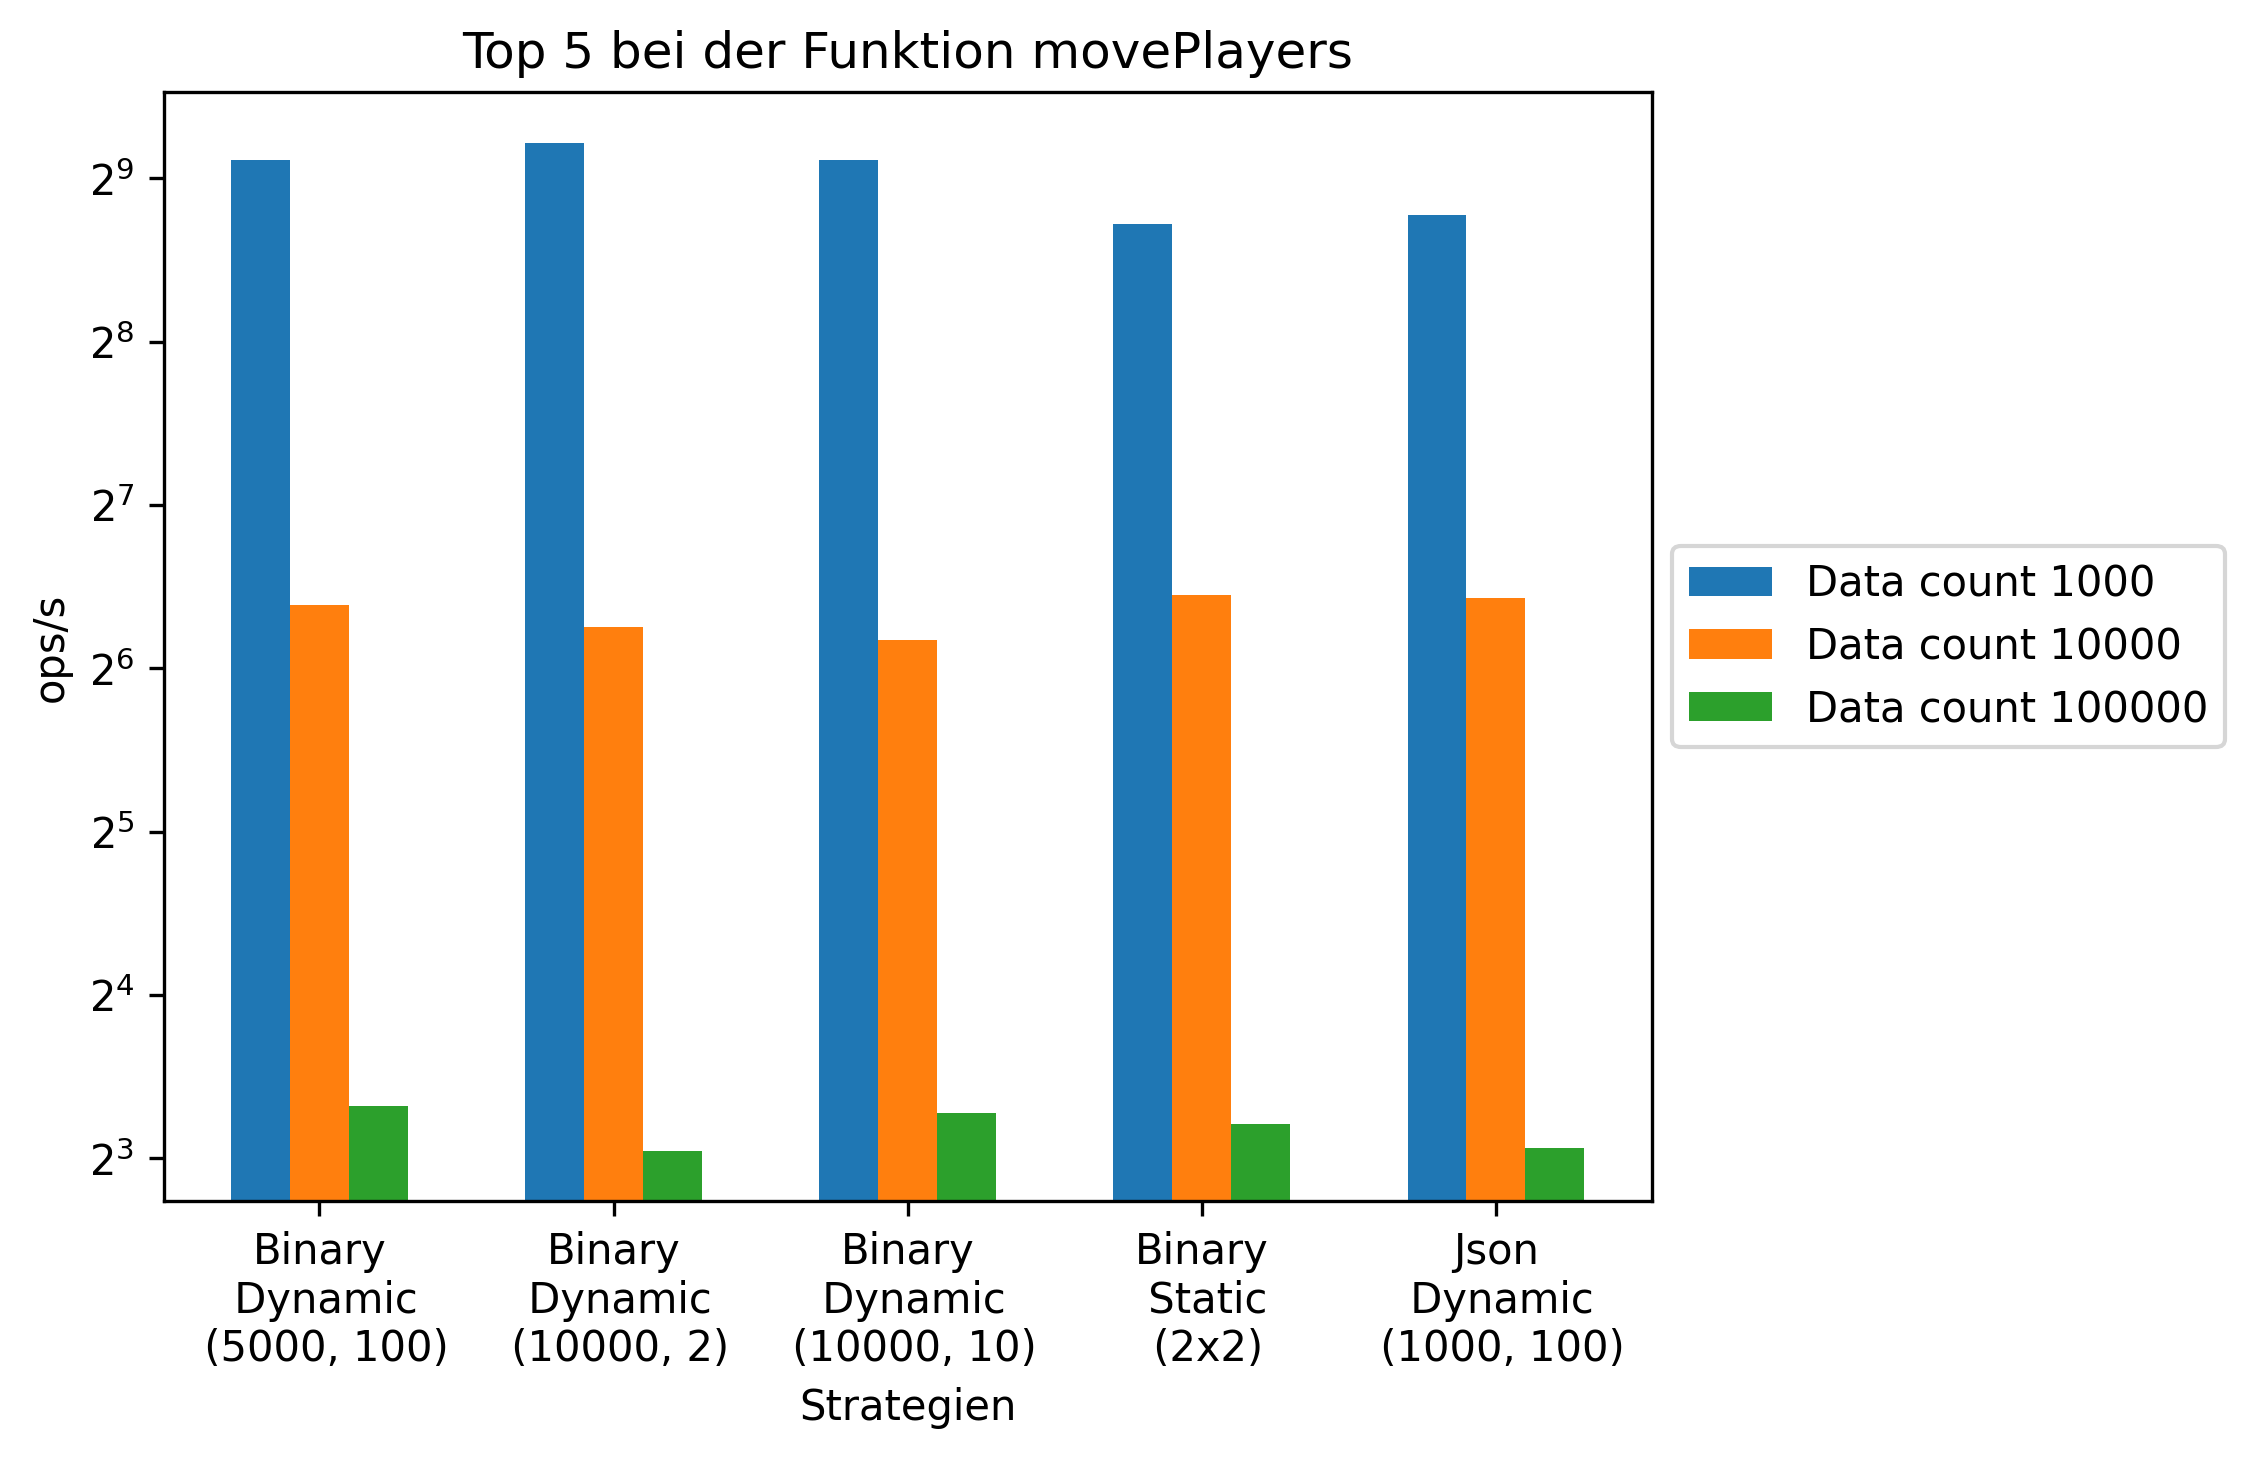
\includegraphics[width=0.7\textwidth]{images/plots/movePlayers.png}
    \caption{Beste Strategien für die Funktion movePlayers}
    \label{fig:movePlayers}
\end{figure}

\begin{figure}[htp]
    \centering
    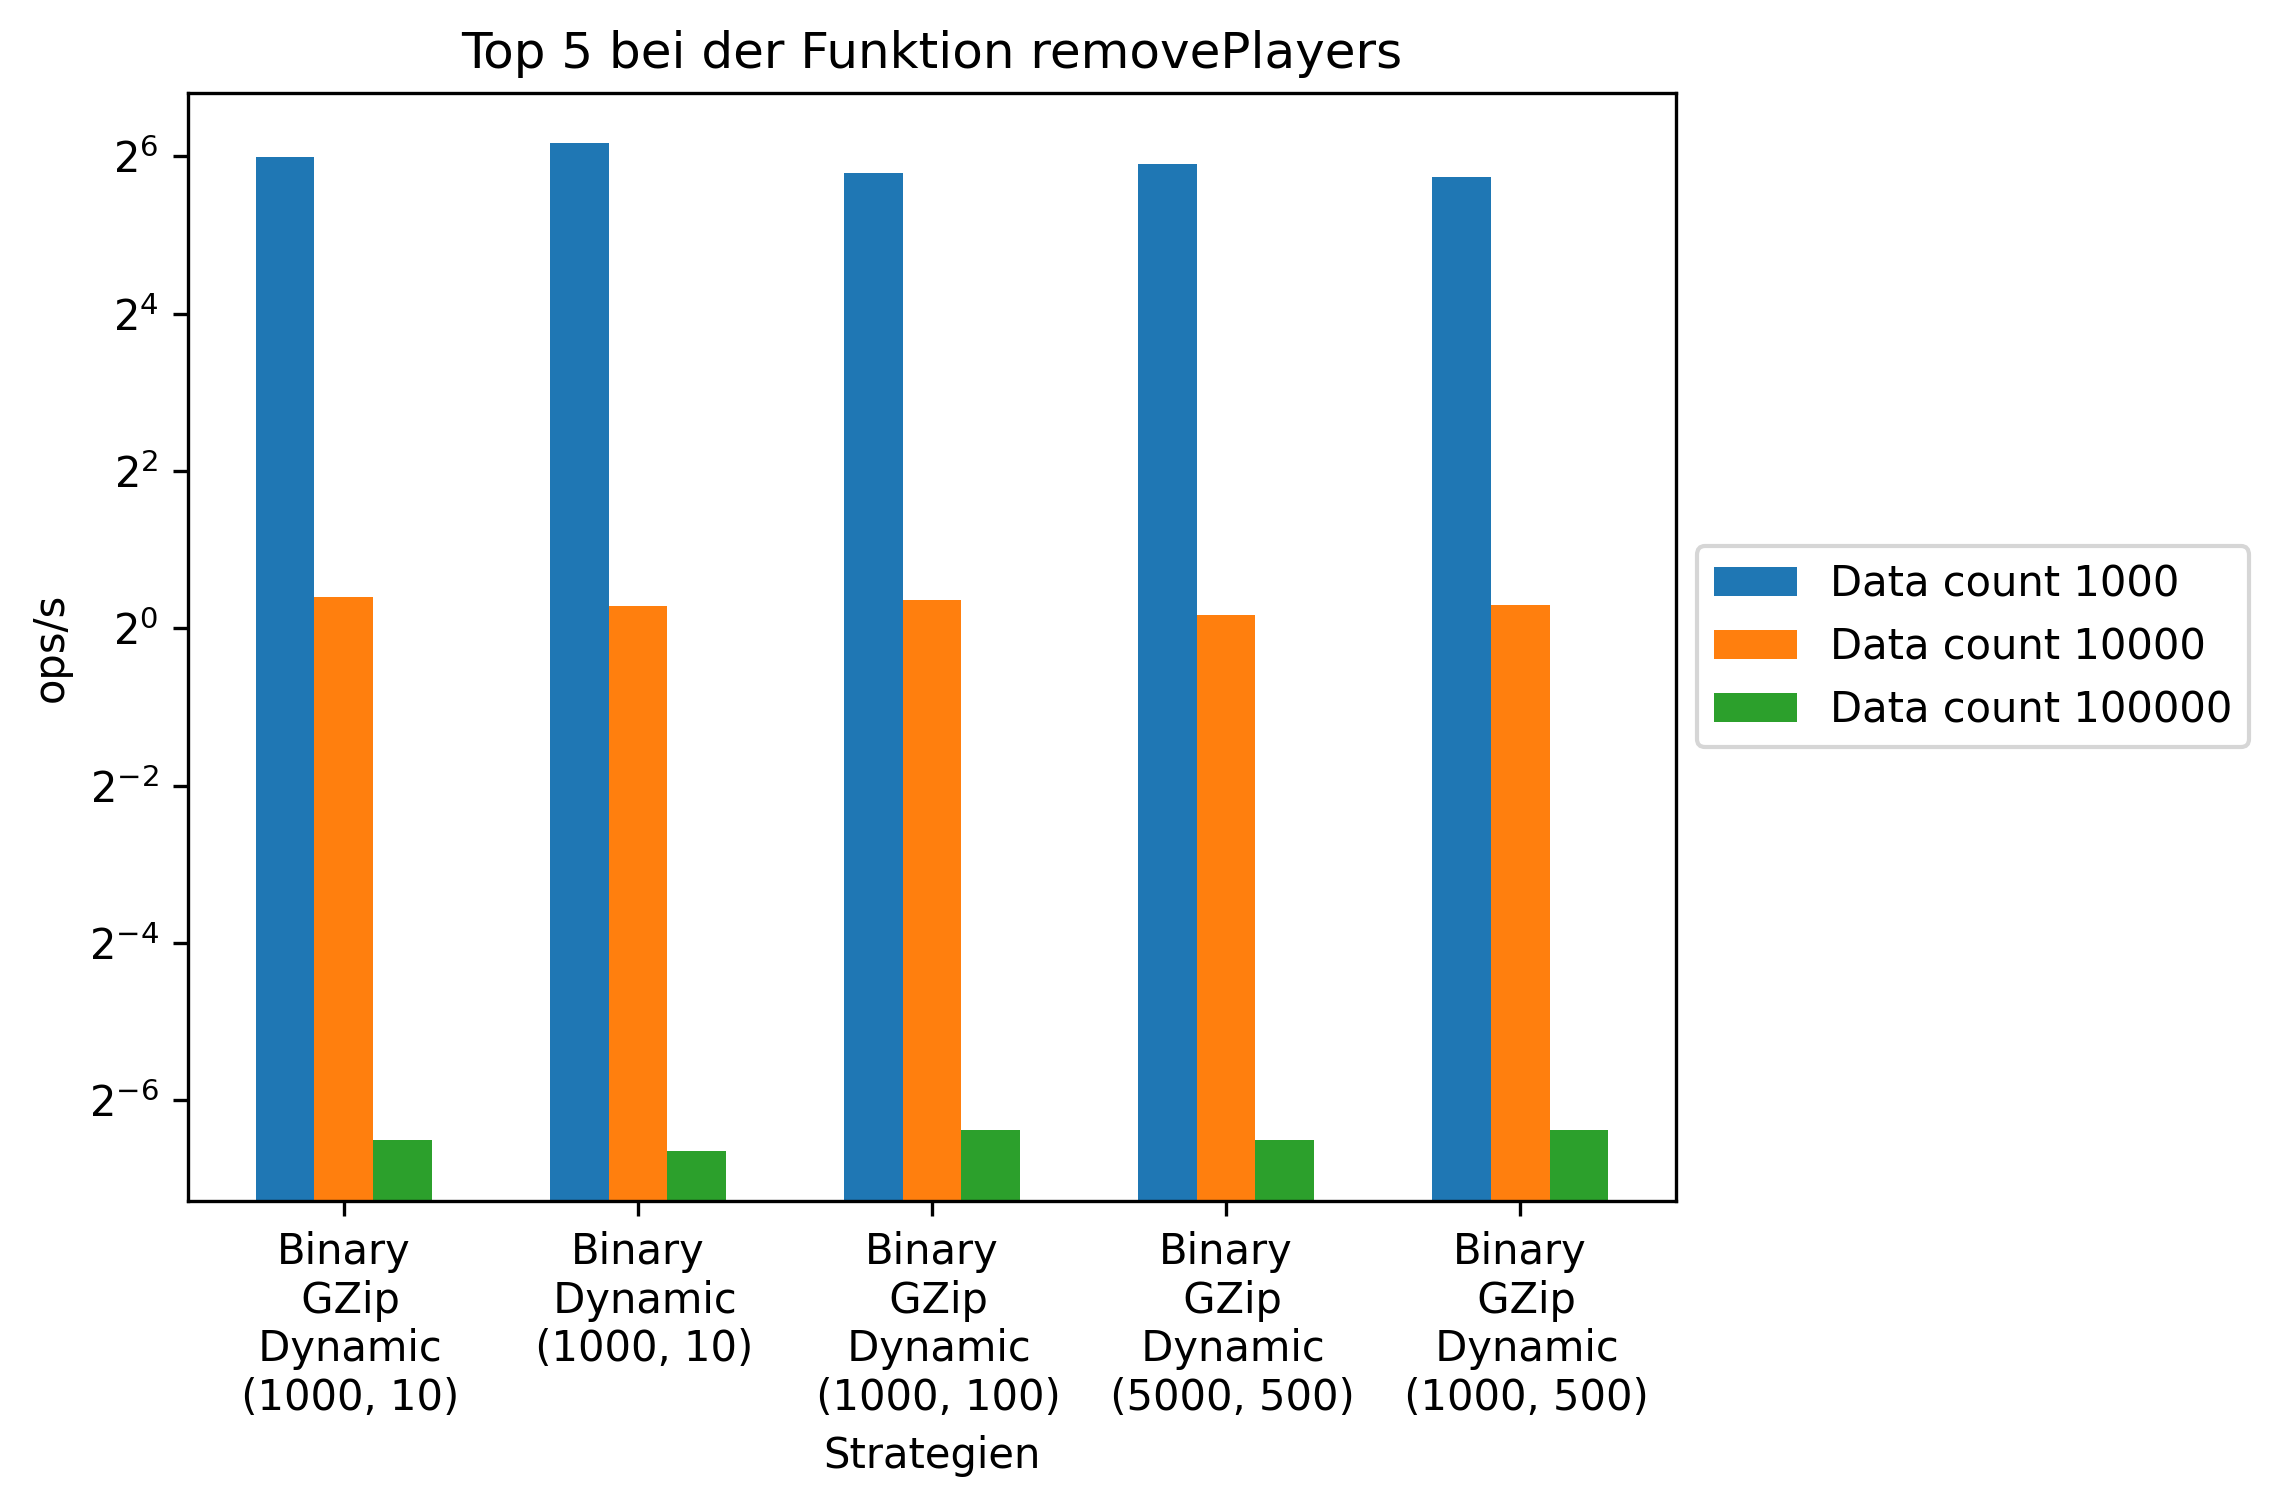
\includegraphics[width=0.7\textwidth]{images/plots/removePlayers.png}
    \caption{Beste Strategien für die Funktion removePlayers}
    \label{fig:removePlayers}
\end{figure}

\begin{figure}[htp]
    \centering
    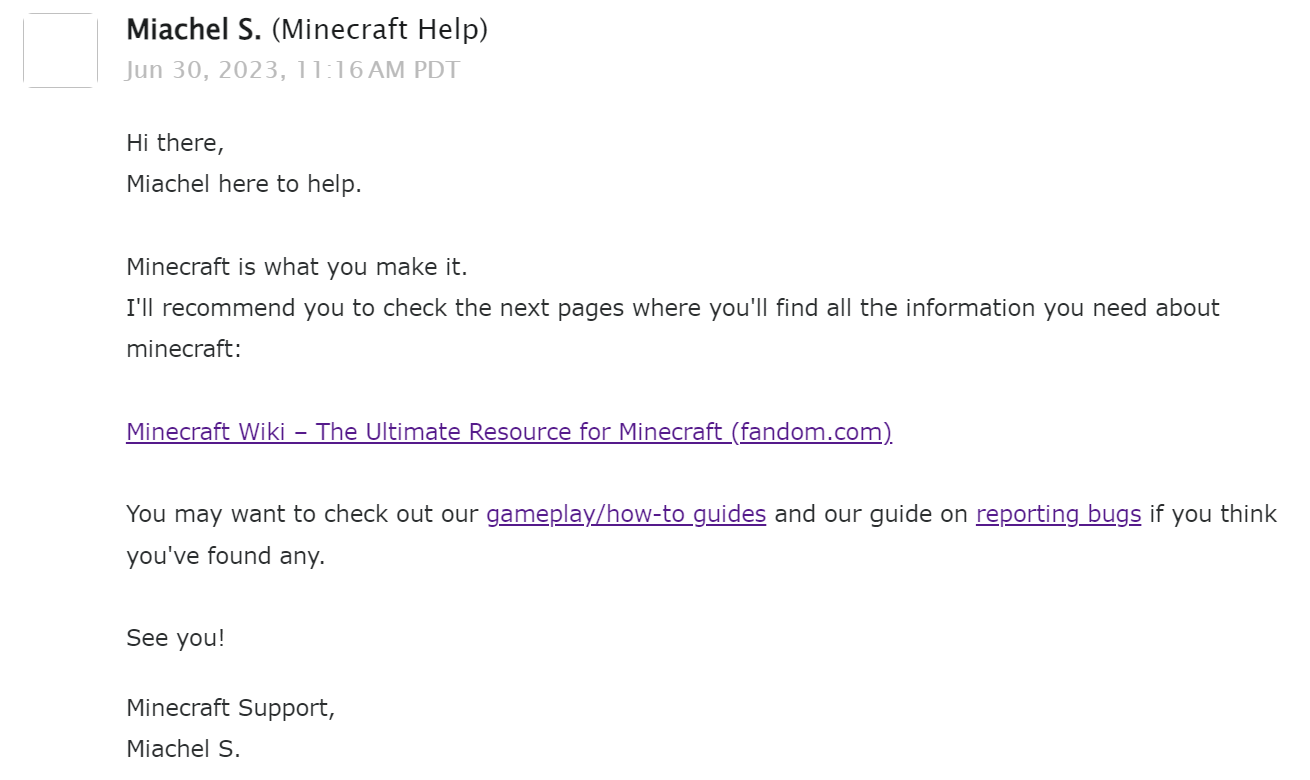
\includegraphics[width=1\textwidth]{images/Minecraft_Email.png}
    \caption{Email von Minecraft zu dem Speicher- und Ladesystem}
    \label{fig:minecraftMail}
\end{figure}

\begin{figure}[htp]
    \centering
    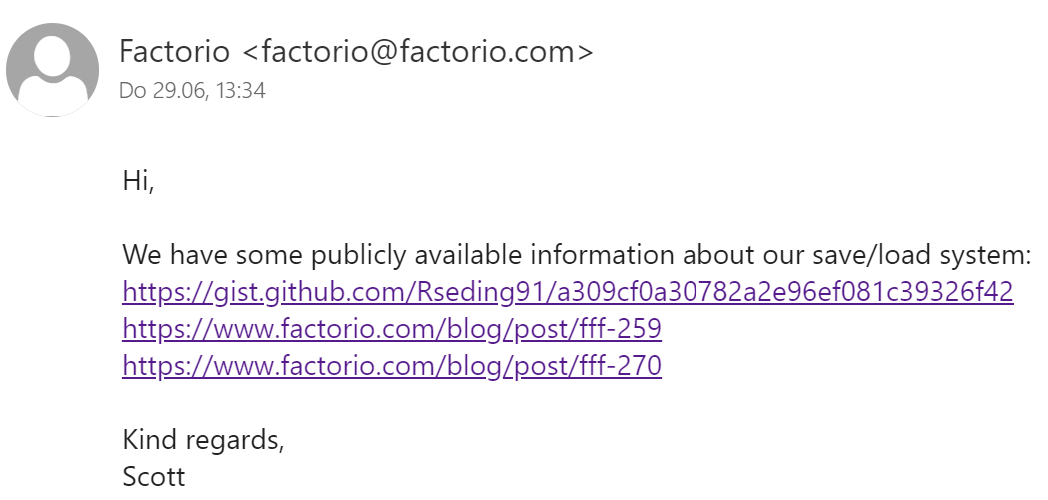
\includegraphics[width=1\textwidth]{images/Factorio_Email.png}
    \caption{Email von Factorio zu dem Speicher- und Ladesystem}
    \label{fig:factorioMail}
\end{figure}
